\documentclass[12pt]{article}
\usepackage{amsmath}
\usepackage[margin=1in]{geometry}
\usepackage[makeroom]{cancel}

\usepackage{amssymb}
\usepackage{graphicx}

\title{Homework 1: Problem 4}
\author{David Denberg}
\date{\today}

\begin{document}
\maketitle
\noindent
\textbf{Part A}
\begin{align*}
f(x) &= 1 - e^{-x}
\\
f'(x) &= e^{-x}
\\
(\mathrm{cond} \; f)(x) &= \bigg|\frac{x f'(x)}{f(x)}\bigg| = \bigg|\frac{x e^{-x}}{1 - e^{-x}}\bigg| = \frac{x e^{-x}}{1 - e^{-x}} \quad \mathrm{on} \; x \in (0,1)
\end{align*}
To show $(\mathrm{cond} \; f)(x)$ is less then 1 on (0,1), we first assume:
\begin{align*}
\frac{x e^{-x}}{1 - e^{-x}} &< 1
\\
x e^{-x} &< 1 - e^{-x}
\\
x &< e^x - 1 = x + \frac{x^2}{2!} + \frac{x^3}{3!} + ... 
\\
0 &< \frac{x^2}{2!} + \frac{x^3}{3!} + ...
\end{align*}
This last expression is true for $x \in (0,1)$, so $(\mathrm{cond} \; f)(x) < 1$ on (0,1).

\noindent
\textbf{Part B}
\begin{align*}
\mathrm{fl}(e^{-x}) &= e^{-x} (1 + \epsilon_{exp})
\\
\mathrm{fl}(1 - \mathrm{fl}(e^{-x})) &= \mathrm{fl}\bigg((1 - e^{-x}) \bigg(1 + \frac{\epsilon_1}{1 - e^{-x}} - \frac{\epsilon_{exp} e^{-x}}{1 - e^{-x}}\bigg)\bigg)
\\
f_A(x) &= (1 - e^{-x}) \bigg(1 + \frac{\epsilon_1}{1 - e^{-x}} - \frac{\epsilon_{exp} e^{-x}}{1 - e^{-x}} + \epsilon_{rnd}\bigg)
\end{align*}
To get an upper bound on the error we let $\epsilon_1 = \epsilon_{rnd} = -\epsilon_{exp} = \mathrm{eps}$. Then the maximum bounded $f_A(x)$ is:
\begin{align*}
f_A(x) &= (1 - e^{-x}) \bigg(1 + \frac{2 \cdot \mathrm{eps}}{1 - e^{-x}}\bigg) = 1-e^{-x}+2\cdot \mathrm{eps}
\end{align*}
The condition of the algorithm is calculated as:
\begin{align*}
(\mathrm{cond} \; A)(x) = \frac{1}{\mathrm{eps}} \bigg| \frac{x_A - x}{x} \bigg| = \frac{1}{\mathrm{eps}} \bigg| \frac{-\ln(1 - f_A(x)) - x}{x} \bigg|
\end{align*}
First we plug in $f_A(x)$ into the expression:
\begin{align*}
\frac{1}{\mathrm{eps}} \bigg|\frac{-\ln(1-1+e^{-x}-2\cdot \mathrm{eps}) - x}{x} \bigg| &= \frac{1}{\mathrm{eps}} \bigg|\frac{-\ln(e^{-x}(1-2\cdot \mathrm{eps} \cdot e^x)) - x}{x} \bigg|
\\
&= \frac{1}{\mathrm{eps}} \bigg|\frac{x-\ln(1-2\cdot \mathrm{eps} \cdot e^x) - x}{x} \bigg|
\\
&= \frac{1}{\mathrm{eps}} \bigg|\frac{-\ln(1-2\cdot \mathrm{eps} \cdot e^x)}{x} \bigg|
\end{align*}
For eps $\ll 1$ we can expand the logarithm:
\begin{align*}
\frac{1}{\mathrm{eps}} \bigg|\frac{2\cdot \mathrm{eps} \cdot e^x + \cancelto{\approx 0}{2 \cdot \mathrm{eps}^2 \cdot e^{2x}} + ...}{x} \bigg| &= \frac{1}{\mathrm{eps}} \bigg|\frac{2\cdot \mathrm{eps} \cdot e^x}{x} \bigg|
\\
&= \frac{2 e^x}{x}
\end{align*}
on (0,1). Thus $(\mathrm{cond} \; A)(x)$ is bounded by $\frac{2 e^x}{x}$ which is always greater than 1 on (0, 1).

\noindent
\textbf{Part C}

\begin{figure}[!h]
\centering
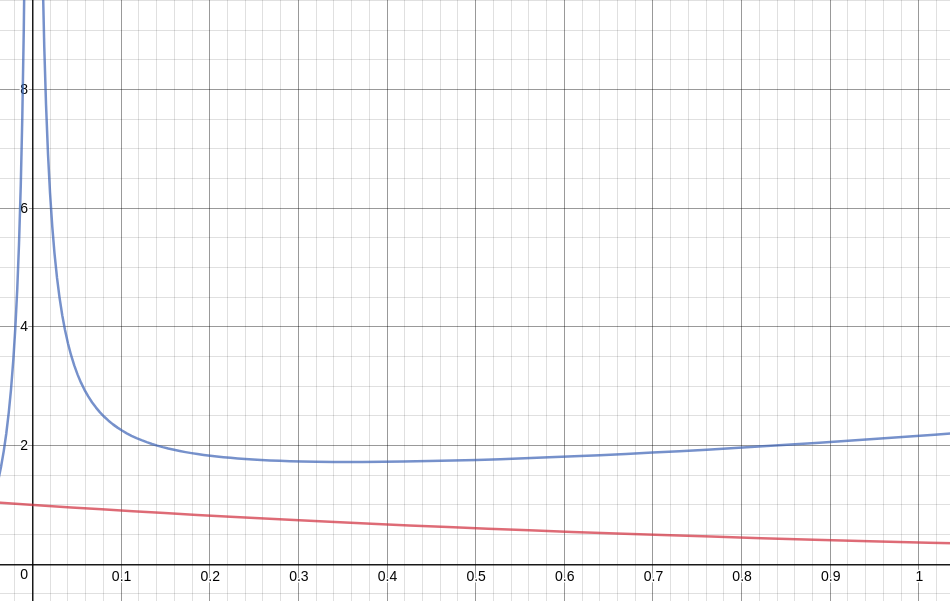
\includegraphics[width=0.5\textwidth]{plot_condA.png}
\caption{$(\mathrm{cond} \; f)(x)$ is in red and $(\mathrm{cond} \; A)(x)$ is in blue}
\end{figure}
The cause of the poor conditioning when x becomes small in $(\mathrm{cond} \; A)(x)$ is the floating point error due to subtraction.

\noindent
\textbf{Part D}

To find the value of x at which b bits of significance are lost we use the upper bounded $f_A(x)$:
\[
f_A(x) = (1 - e^{-x}) \bigg(1 + \frac{2 \cdot \mathrm{eps}}{1 - e^{-x}}\bigg)
\]
And
\[
\epsilon_{max} = \frac{2 \cdot \mathrm{eps}}{1 - e^{-x}}
\]
Is the maximum error. Then for b bits of significance lost:
\begin{align*}
\log_2\bigg( \frac{2 \cdot \mathrm{eps}}{1 - e^{-x}}\bigg) &= b
\\
x &= -\log \bigg(1 - \frac{\cdot \mathrm{eps}}{2^{b-1}}\bigg)
\end{align*}
For 1, 2, 3, and 4 bits lost we need:
\begin{align*}
x_1 &= -\log \bigg(1 - \mathrm{eps}\bigg)
\\
x_2 &= -\log \bigg(1 - \frac{\mathrm{eps}}{2}\bigg)
\\
x_3 &= -\log \bigg(1 - \frac{\mathrm{eps}}{4}\bigg)
\\
x_4 &= -\log \bigg(1 - \frac{\mathrm{eps}}{8}\bigg)
\end{align*}

\noindent
\textbf{Part E}

The maximum relative error is:
\[
\frac{2 \cdot \mathrm{eps}}{x(1 - e^{-x})}
\]

\noindent
\textbf{Part F}

An alternative function to evaluate would be:
\[
f(x) = \ln \bigg(\frac{e}{e^{e^{-x}}} \bigg)
\]
Because there isn't subtraction present then there shouldn't be a source of floating point error when x goes to 0.



\end{document}